\documentclass[11pt,letterpaper]{article}
\usepackage[top=1in,bottom=1in,left=1in,right=1in]{geometry}
\pagestyle{empty}
\usepackage{graphicx}
\usepackage{amsmath}

\usepackage[dvipsnames]{xcolor}
%\newcommand{\sol}[1]{{\color{NavyBlue} #1}}
\newcommand{\sol}[1]{{\color{White} #1}} % uncomment to hide solutions


\begin{document}
\setlength{\parindent}{0cm}
\setlength{\parskip}{11pt}
Exam \#1: Basic kinematics and dynamics

Name: \hfill /30\\

\hrulefill\\
1. Conceptual problems

a. The velocity-time graph of a car is shown below. During each of the four time intervals, indicate whether the car is speeding up or slowing down. [4 pts]
\begin{figure}[h]
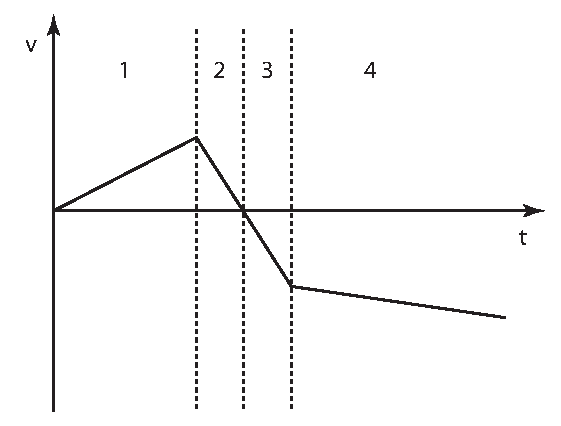
\includegraphics[]{./exam1_1a}
\end{figure}

\sol{Speeding up during periods 1, 3, and 4. In 1 the speed is increasing in the positive direction, and in 3 and 4 the speed is increasing in the negative direction. 

Slowing down during period 2. The speed is decreasing in the positive direction.} 
\vspace{1cm}

b. Three forces acting on an object are indicated by the free-body diagram below. Sketch the net force acting on the object. [3 pts]
\begin{figure}[h]
\centering
%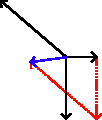
\includegraphics[height=4.5cm]{./exam1_1b_sol}
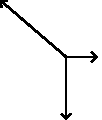
\includegraphics[height=4.5cm]{./exam1_1b}
\end{figure}

c. Draw free-body diagrams for each of the following: (i) a projectile in motion in the presence of air resistance, (ii) a rocket leaving the launch pad with its engines operating, and (iii) an athlete
running along the end of a horizontal track (i.e., as their direction is changing). [3 pts]

%\begin{figure}[h]
%\centering
%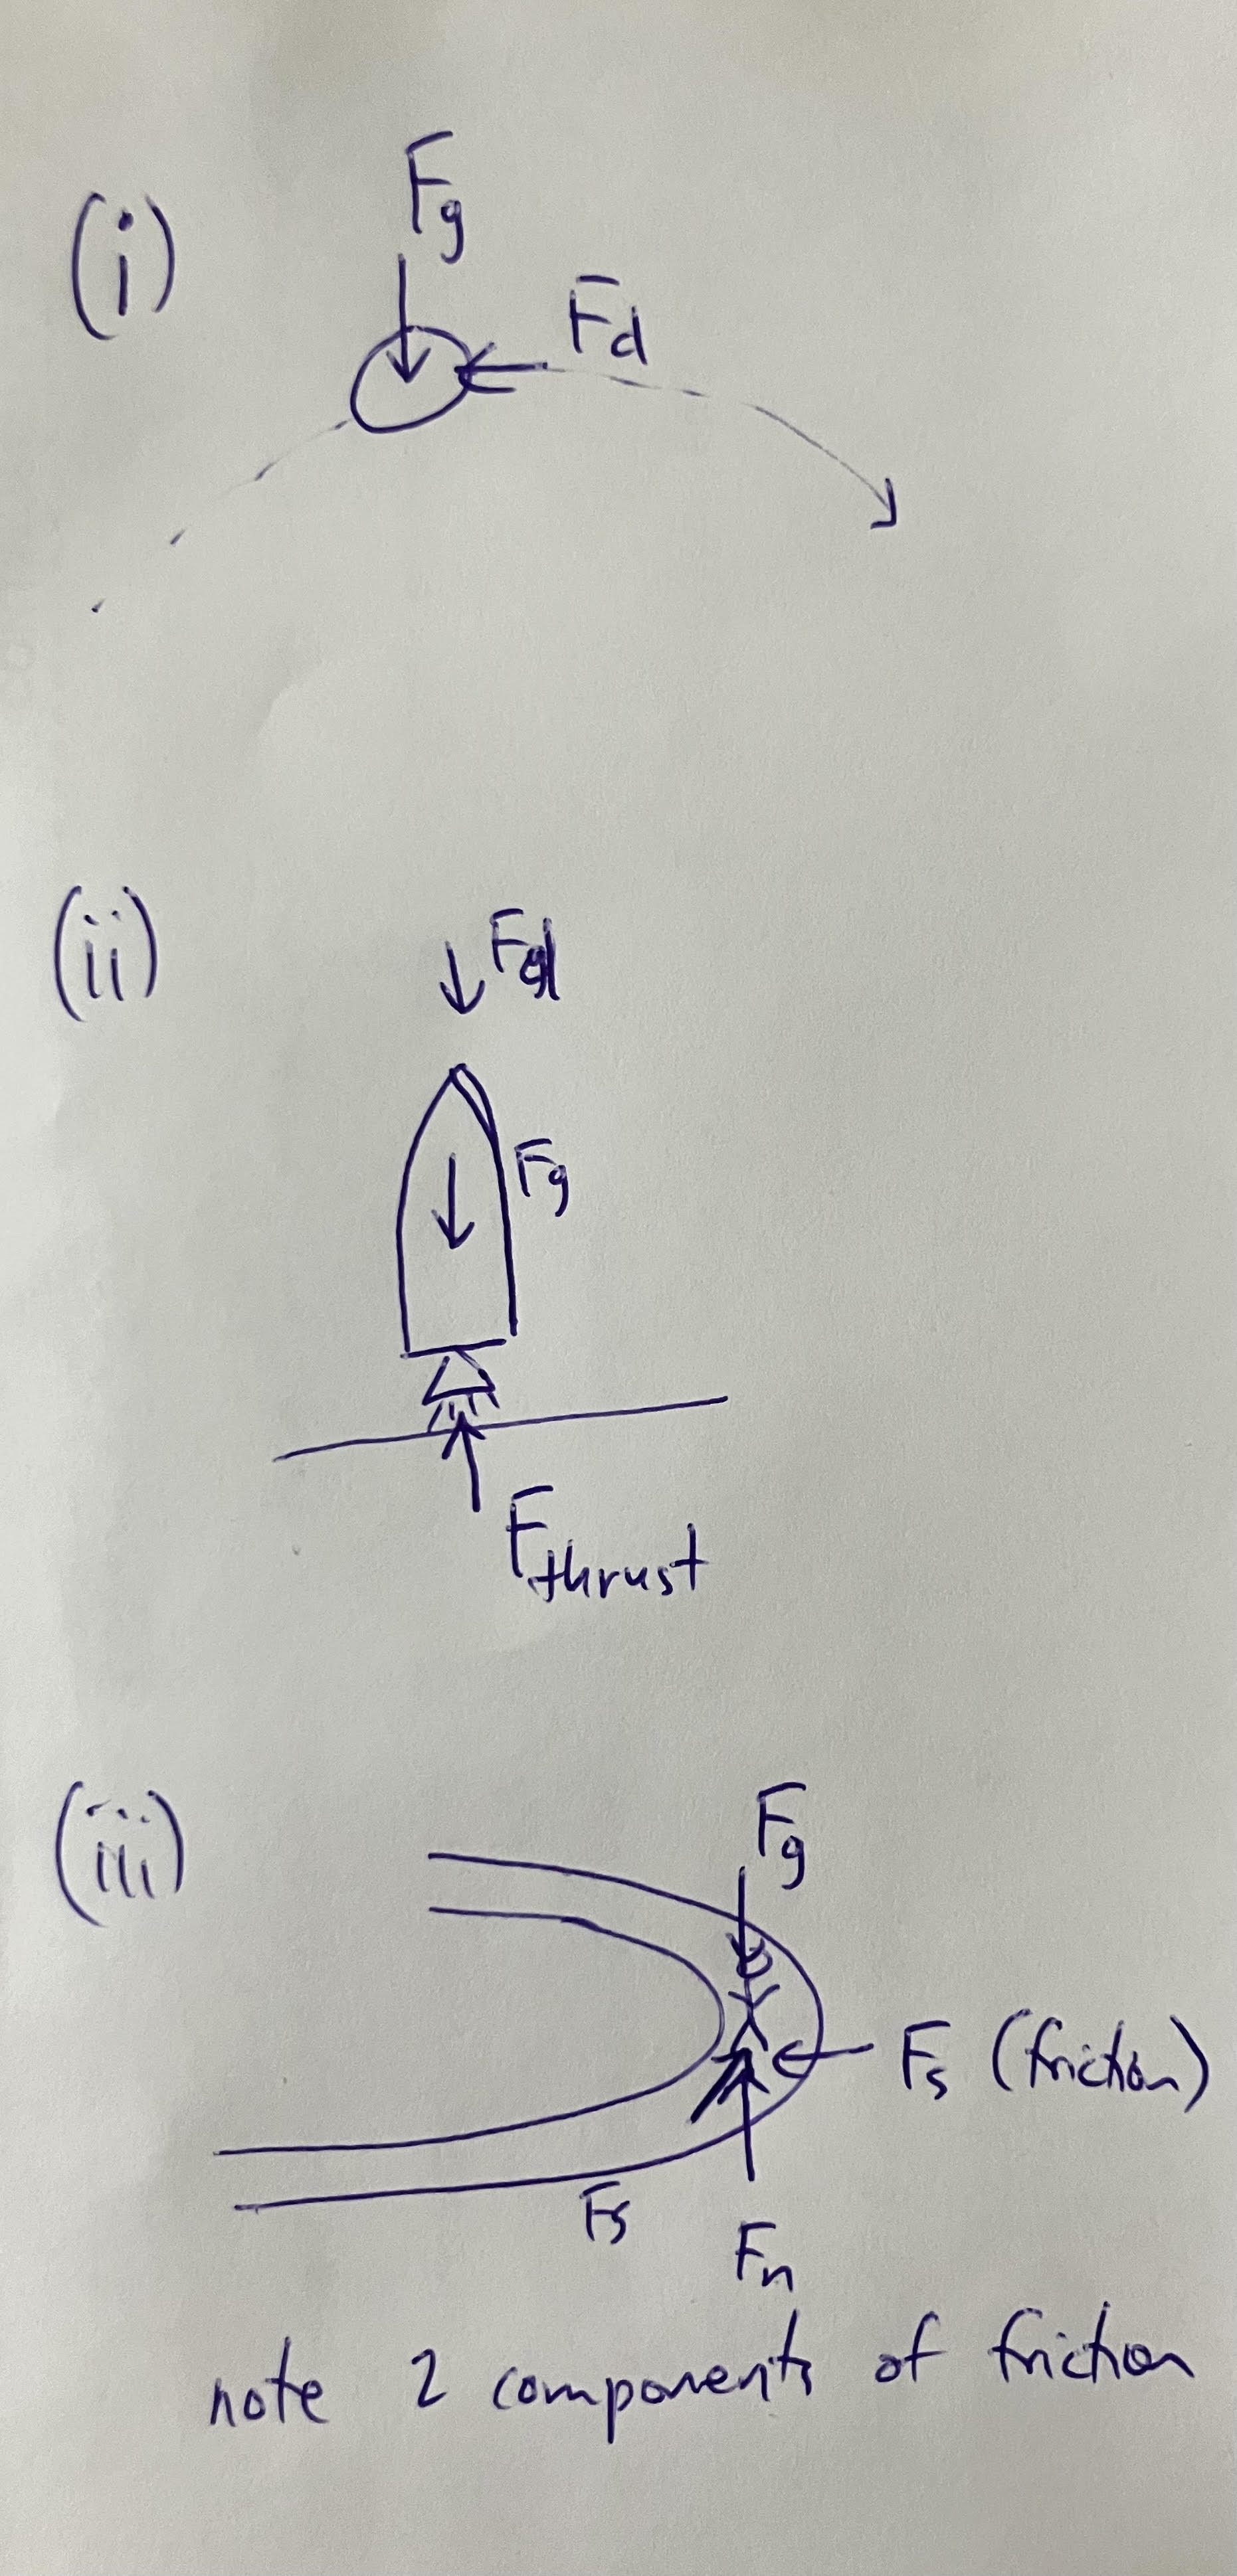
\includegraphics[width=0.5\textwidth]{./exam1_1c.jpg}
%\end{figure}


\clearpage
2. A wrecking ball is hanging from a crane when the cable suddenly breaks. It takes the ball 1.2 s for the ball
to travel halfway to the ground. Ignore air resistance.

a. How far does the ball fall? [3 pts]

\sol{Find the distance that it travels in the first 1.2~s and then multiply by 2.

Given/implied:
$$v_{y,i}=0$$
$$a_y = -g = -9.81\mbox{ m/s}^2$$
$$\Delta t = 1.2\mbox{ s}$$

From this we calculate
$$\Delta y = v_{y,i}\Delta t + \frac{1}{2}a_y\Delta{t}^2=-7.1\mbox{ m},$$
which means that the ball falls $$\boxed{14.1\mbox{ m}}$$.
}
\vspace{2cm}

b. What is the ball’s velocity just before it hits the ground? (3 pts)

\sol{To answer this, we now need to recognize that $\Delta y=-14.1\mbox{ m}$. We can use
$$v_{y,f}^2 - v_{y,i}^2 = 2a_y\Delta y$$
$$v_{y,f} = \pm \sqrt{2a_y\Delta_y} = \boxed{-16.6\mbox{ m/s}}$$

}



\clearpage
3. A Ferris wheel carries its riders in a (vertically oriented) circle with a radius of 8.0 m. The Ferris wheel makes one revolution every 9.0 s. 

a. Calculate the angular velocity. [2 pts]

\sol{$$\omega = 2\pi f = \frac{2\pi}{T} = \boxed{0.70\mbox{ rad/s}}$$}
\vspace{1cm}

b. Calculate the centripetal acceleration and centripetal force acting on a 70-kg person as they travel around in a circle on the Ferris wheel. What direction does the force point? [2 pts]

\sol{
$$a_c = \omega^2r = \boxed{3.9\mbox{ m/s}^2}$$
$$F_c = ma_c = \boxed{272\mbox{ N, directed inward}}$$}
\vspace{1cm}


c. What is the person's apparent weight (or normal force acting upward on them) as they pass the lowest point of the circle? How does this compare to their weight? [2 pts]

\sol{
$$\sum F_c = F_n - F_g = ma_c$$
$$F_n = F_g + ma_c = mg+ma_c = m(g+a_c) = \boxed{960\mbox{ N}}$$

Their weight is simply 
$$F_g = mg = \boxed{687\mbox{ N}}$$

}




\clearpage
4. Chinook salmon are able to move upstream faster by jumping out of the water periodically; this behavior is called porpoising. Suppose a salmon swimming in still water jumps out of the water with a speed of 6.26~m/s at an angle of 45$^\circ$, sails through the air a distance $L$ before returning to the water, and then swims a distance $L$ at a speed of 3.58~ m/s before beginning another porpoising maneuver. Determine the average speed of the fish. 

a. How long is the fish in the air during one ``jump''? [2 pts]

\sol{
Given:
$$\Delta y = 0$$
$$v_{y,i} = 6.26\sin(45^\circ)$$
$$a_y = -g = -9.81\mbox{ m/s}^2$$
We can solve this using:
$$\Delta y = v_{y,i}\Delta t + \frac{1}{2}a_y\Delta t^2$$
Setting $\Delta y=0$ and dividing by $\Delta t$,
$$0 = v_{y,i} + \frac{1}{2}a_y\Delta t$$
Solving for $\Delta t$,
$$\Delta t = \frac{-2v_{y,i}}{a_y} = \boxed{0.9\mbox{ s}}$$
}
\vspace{2cm}

b. How far does the fish travel during each ``jump''? [2 pts]

\sol{
$$\Delta x = v_x\Delta t$$
$$v_x = 6.26\cos(45^\circ)$$
Therefore
$$\Delta x = \boxed{4.0\mbox{ m}}$$
} 
\vspace{1cm}

c. How much time does the fish spend in the water between each ``jump''? [2 pts]

\sol{Assume constant speed, and note that $\Delta x = L=4.0$~m and $v=3.58\mbox{ m/s}$.
$$\Delta x = v\Delta t$$
$$\Delta t = \frac{\Delta x}{v} = \boxed{1.1\mbox{ s}}$$
}
\vspace{1cm}

d. What is the average speed of the fish? [2 pts]

\sol{Again assume velocity in the x-direction is constant.
$$v = \frac{\Delta x}{\Delta t}$$
Here, $\Delta x = 2L$ and $\Delta t = 2\mbox{ s}$ (the total time that passes between ``jumps''. This gives
$$\boxed{v = 3.96\mbox{ m/s}}$$
}


\end{document}
